%MIT OpenCourseWare: https://ocw.mit.edu
%RES.18-011 Algebra I Student Notes, Fall 2021
%License: Creative Commons BY-NC-SA 
%For information about citing these materials or our Terms of Use, visit: https://ocw.mit.edu/terms.

\section{Finite and Discrete Subgroups, Continued}

\subsection{Review}
Last time, we began studying certain subgroups of $M_2.$ The group of \emph{isometries} of $\RR^2$ is precisely
\[
M_2 = \{t_{\vv{b}} \circ A : \vv{b} \in \RR^2, A \in O_2\},
\]
where $O_2$ is the group of orthogonal matrices. 

\begin{qq}
What are the finite subgroups of $O_2$?\footnote{The discrete subgroups of $O_2$ turn out to be the same as the finite subgroups, either $C_n$ or $D_n$ (we omit the proof, as it is in the homework.)} 
\end{qq}
One way in which subgroups of $M_2$ naturally arise is with symmetries of plane figures. 
\begin{example}
For the following two plane figures, they both have discrete symmetries including translations, rotations, and glide reflections. 
\begin{center}
    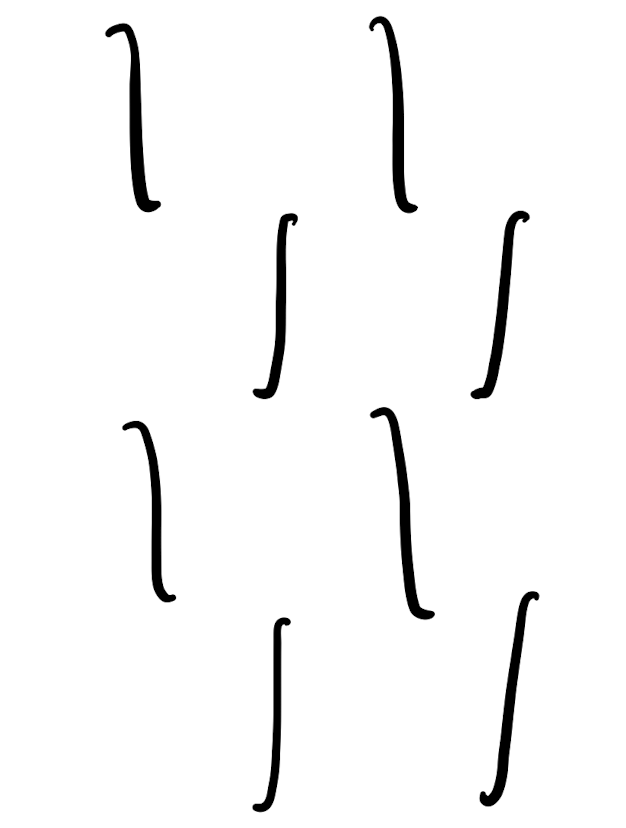
\includegraphics[width=3cm]{Lecture Files and Images/lec15-1integrals.png} 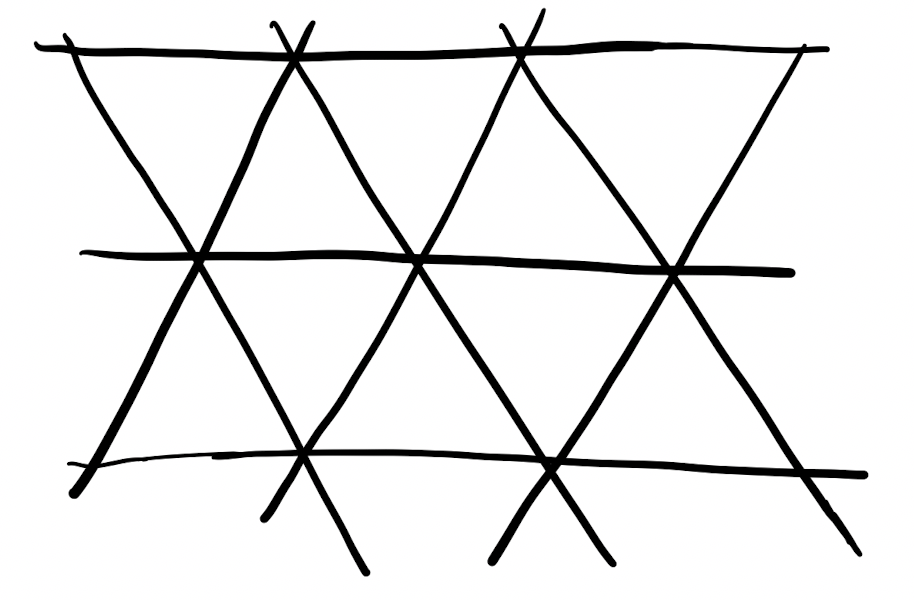
\includegraphics[width=6cm]{Lecture Files and Images/lec15-2trianglegrid.png}
\end{center}
\end{example}

Last time, we looked at finite subgroups of the orthogonal matrices $G \subseteq O_2.$ We found the following theorem which greatly restricts the possibilities for such subgroups:
\begin{theorem}\label{everything is cn or dn}
Any \emph{finite} subgroup $G \subseteq O_2$ is either 
\begin{itemize}
    \item $G \cong C_n = \langle \rho_{2\pi/n} \rangle$, the cyclic group generated by a \emph{rotation} by $2\pi/n$; or
    \item $G\cong D_n = \langle \rho_{2\pi/n}, r \rangle $ which is the group $C_n$ with an extra reflection $r.$  
\end{itemize}
\end{theorem}

The elements of the form $\rho_{2\pi/n}$, which are rotations by $2\pi/n,$ are orientation-preserving, while elements of the form $\rho_{2\pi / n}r$, which are reflections over certain lines through the origin, are orientation-reversing.


\subsection{Finite Subgroups of \texorpdfstring{$M_2$}{M2}}

Now that we have found the finite and discrete subgroups of $O_2,$ we bring our attention to finite subgroups $G \subseteq M_2.$
\begin{qq}
What are the finite subgroups of $M_2$? Do we get more subgroups now that we have more elements?
\end{qq}

In fact, there are \emph{no} new finite subgroups obtained from allowing $G$ to be in $M_2$ instead of $O_2.$ 

\begin{theorem}
Any finite subgroup $G \subseteq M_2$ is also isomorphic to $C_n$ or $D_n.$
\end{theorem}

\begin{proof}
In order to show that $G$ is isomorphic to $C_n$ or $D_n$, it is enough to find $s_0 \in \RR^2$ such that $g(s_0) = s_0$ for all $g \in G.$ Then, by changing coordinates such that $s_0$ is the new origin\footnote{We take $t_{-s_0}Gt_{s_0}$}, $G$ fixes the origin (formerly $s_0$) and so $G \subseteq O_2.$ As a result, by applying Theorem \ref{everything is cn or dn}, $G$ must in fact be isomorphic to $C_n$ or $D_n.$

\begin{itemize}
    \item \textbf{Step 1.} First, we find some finite set $S$ fixed by every element $g$: we require that $gS = S$ for all $g \in G.$ For any $p \in \RR^2,$ let 
    \[
    S = \{g(p) \in \RR^2: g \in G\}\footnote{This is called the \emph{orbit} of $p,$ since it is all the points that $p$ can reach by some transformation in $G$, or all the points that $p$ orbits to.}.%somehow this doesn't seem right in wording
    \]
    
    Then, for any element $s \in S,$ it is equal to $s = g'(p)$ for some $g' \in G,$ by the definition of $S.$ In addition, for any $g \in G,$ the action of $g$ on $s$ is
    \[
    g(s) = g(g'(p')) = (gg')(p) \in S,
    \]
    again by how $S$ is defined. So 
    \[
    gS = S.
    \]
    
    \item \textbf{Step 2.} Intuitively, to find $s_0,$ we would take the average, or the center of mass, of all the points. For example, for the set of rotations $\langle 2\pi/3\rangle,$ $S$ would be 3 equidistant points, and the center of the equilateral triangle would be fixed by such rotations. 
    From this intuition, we can apply the following averaging trick. This is where $G$ being finite is required, as we wouldn't be able to take the average otherwise. %ask davesh more about averaging to put in a footnote?
    
    Where $S = \{s_1, \cdots, s_n\}$, let
    \[
    s_0 = \frac{1}{n}(s_1 + \cdots + s_n)
    \]
    be the average of all the elements in $S.$ For any isometry $f = t_b \circ A,$ 
    \begin{align*}
    f(s_0) &= t_b\left(\frac{1}{n}(As_1 + \cdots + As_n)\right) \\
    &= \frac{1}{n}((As_1 + b) + \cdots + (As_n + b)) \\
    &= \frac{1}{n}(f(s_1) + \cdots + f(s_n)),
    \end{align*}
    since $A$ is a linear operator.
    
    As a result, for any $g \in G,$ 
    \begin{align*}
    g(s_0) &= \frac{1}{n}(g(s_1) + \cdots + g(s_n)) \\
    &= \frac{1}{n}(s_1 + \cdots + s_n) \\
    &= s_0,
    \end{align*}
    since $g$ permutes the elements in $S$.%why does it do that again lmao
    
    So we see that $G$ does fix $s_0,$ and by changing coordinates so that $s_0$ is the origin, $G$ must in fact be isomorphic to $C_n$ or $D_n.$
\end{itemize}
\end{proof}

\subsection{Discrete Subgroups of \texorpdfstring{$M_2$}{M2}}

No new finite subgroups are obtained by taking elements in $M_2$ instead of $O_2;$ what if we take discrete subgroups\footnote{We will formalize the notion of discreteness in $M_2$ now!} instead of finite subgroups? 

\begin{qq}
What about discrete subgroups of $M_2$? 
\end{qq}

The definition of discreteness in $M_2$ combines the two definitions for the rotations and translations.
\begin{definition}
A group $G \subseteq M_2$ is discrete if there exists some $\varepsilon > 0$ such that any translation in $G$ has distance $\geq \varepsilon$ and any rotation in $G$ has angle $\geq \varepsilon.$\footnote{In fact, for discreteness, it would make more sense to require two different $\varepsilon_1$ and $\varepsilon_2$ for translations and rotations, just to ensure that there are not continuously many translations and rotations. In this case, we can simply acquire the $\varepsilon$ for this definition by taking the minimum of the two; then any translation in $G$ has distance $\geq \varepsilon_1 \geq \varepsilon$ and any rotation has angle $\geq \varepsilon_2 \geq \varepsilon.$}

\begin{center}
    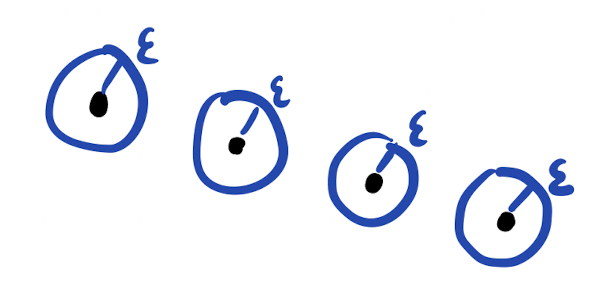
\includegraphics[width=5cm]{Lecture Files and Images/lec15-balls.png}
\end{center}
\end{definition}


\subsubsection{Discrete Subgroups of \texorpdfstring{$\RR^2$}{R2}}

As a warmup, let's consider the copy of the plane inside $M_2,$ $(\RR^2, +) \subseteq M_2,$ consisting of the translations $t_b.$ What are the discrete subgroups of $(\RR^2, +)$? The result and argument is similar to the discrete subgroups of $(\RR, +)$ that we covered last week. 

\begin{theorem}\label{discrete sub of r2}
If $G \subseteq \RR^2$ is discrete, then 
\begin{enumerate}
    \item G = \{0\}; or
    \item there exists some $\vec{\alpha} \in \RR^2$ such that $G = \ZZ \vec{\alpha};$ or
    
\begin{center}
    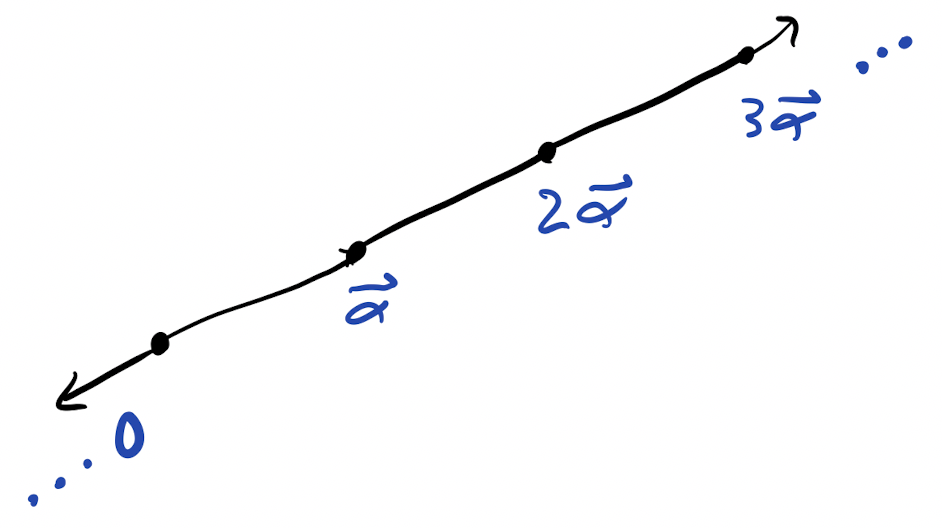
\includegraphics[width=5cm]{Lecture Files and Images/lec16-line.png}
\end{center}
    \item there exist linearly independent vectors $\vec{a}, \vec{b} \in \RR^2$ such that $G = \ZZ \vec{a} + \ZZ \vec{b}.$ This is called a \emph{lattice} inside $\RR^2.$
\begin{center}
    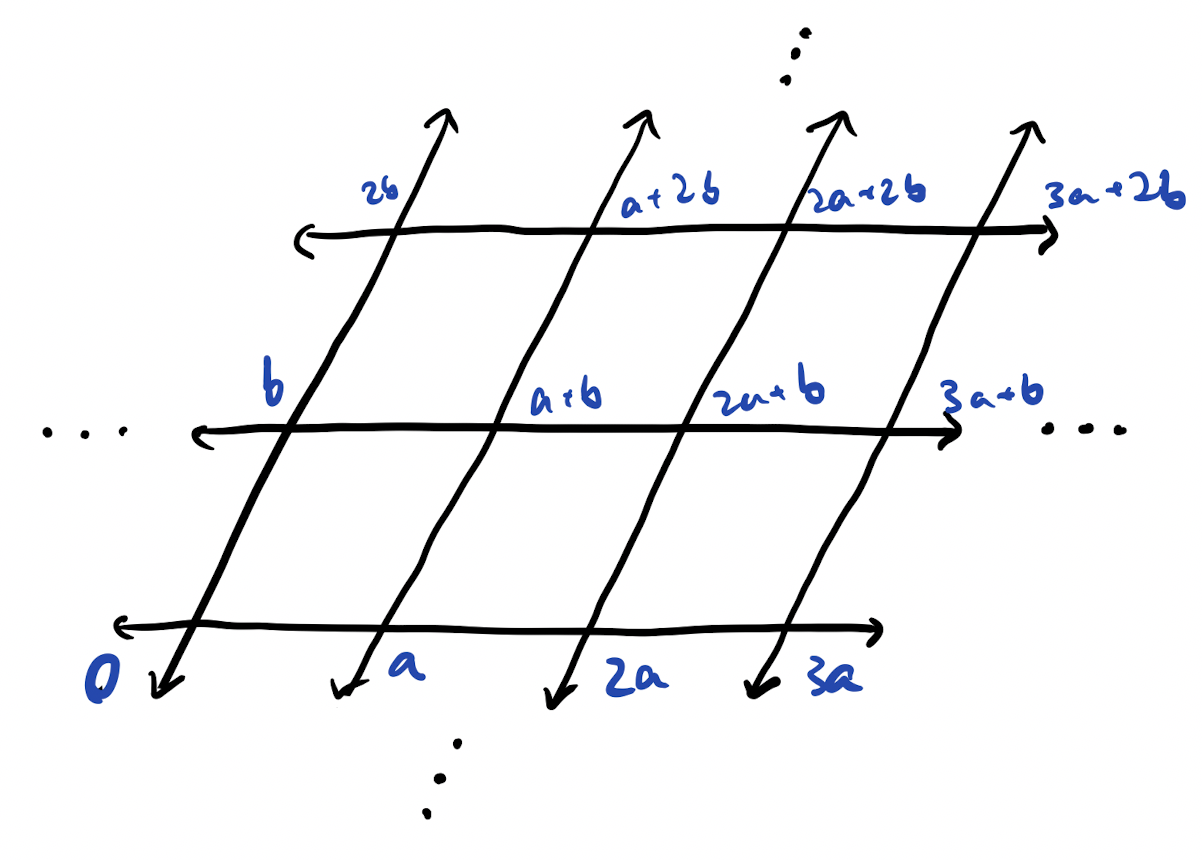
\includegraphics[width=5cm]{Lecture Files and Images/lec15-lattice.png}
\end{center}
\end{enumerate}
\end{theorem}

\begin{proof}
First pick any $\hat{\alpha} \neq 0 \in G.$ The intersection $G \cap \RR\hat{\alpha}$ must be discrete, so there is some smallest length vector in $G \cap \RR\hat{\alpha}$; call it $\alpha.$ Then if $G \cap \RR\hat{\alpha} = G,$ then $G \cap \RR\hat{\alpha} = \ZZ\alpha,$ and we are done. %why is this true?

Otherwise, pick $\beta \in G$ such that $\beta \notin \RR\alpha$, minimizing the distance from $\beta$ to $\RR\alpha.$ There exists such a $\beta$ because in any bounded region of $\RR^2,$ there can only be finitely many points of $G;$ then we can simply pick the point in $G$ closest to $\RR\alpha.$ 

\textbf{Claim: $G = \ZZ\alpha + \ZZ\beta.$} If this were not true, then there would exist a point $\gamma \in G$ that is not on the lattice formed by $\alpha$ and $\beta.$ Thus, by shifting by $\alpha$ and $\beta,$ the parallelogram with sides $\alpha$ and $\beta$ would contain a point closer to $\RR\alpha$, violating the minimality of $\beta$. 
\end{proof}

\subsubsection{Back to Discrete Subgroups of \texorpdfstring{$M_2$}{M2}!}

Now that we have considered the translations in $M_2,$ which are isomorphic to the plane $\RR^2,$ we can move on to the entire $M_2.$
\begin{qq}
How can we study discrete groups $G \subseteq M_2$?
\end{qq}

Recall that there exists a projection $\pi$ from $M_2$ to $O_2$, where $\RR^2,$ the group of translations, is the kernel. The projection takes 
\begin{align*}
    \ker(\pi) = \RR^2 \hookrightarrow\footnote{This arrow often denotes an inclusion map.} &M_2 \xrightarrow[]{\pi} O_2 \\
    &t_{\vv{b}} \circ A \mapsto A.
\end{align*}

The restriction of $\pi$ to $G$ takes $\pi|_G: G \rto O_2.$ The kernel $L = \ker(\pi|_G)$ consists of the translations in $G.$ Under this map, the image of $G$ is a subgroup $\overline{G} \coloneqq \pi(G) \subseteq O_2,$ known as the \textbf{point group} of $G.$ The projection takes
\[
\ker(\pi|_G) = L \subseteq G \xrightarrow[]{\pi|_G} \overline{G}.
\]

\begin{example}
For this infinite plane figure, the group of translations $L$ in the symmetry group $G$ is a rectangular lattice. The point group $\overline{G}$ contains rotation by $\pi$ around $\vv{0}$ and reflection across $\ell;$ as a result, $\overline{G}$ is isomorphic to $D_2.$ 

\begin{center}
    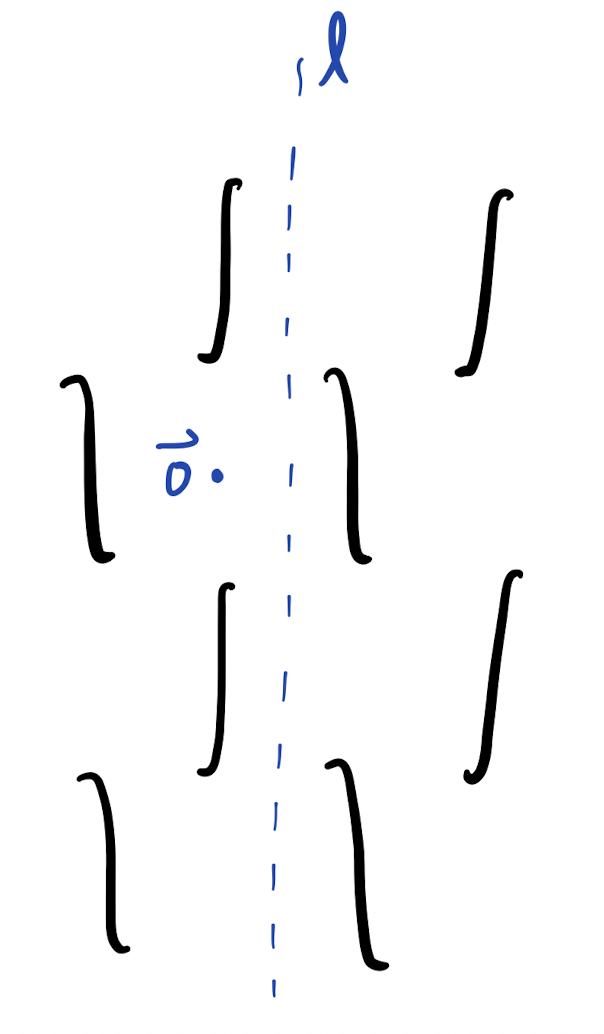
\includegraphics[width=3cm]{Lecture Files and Images/lec15-intl.png}  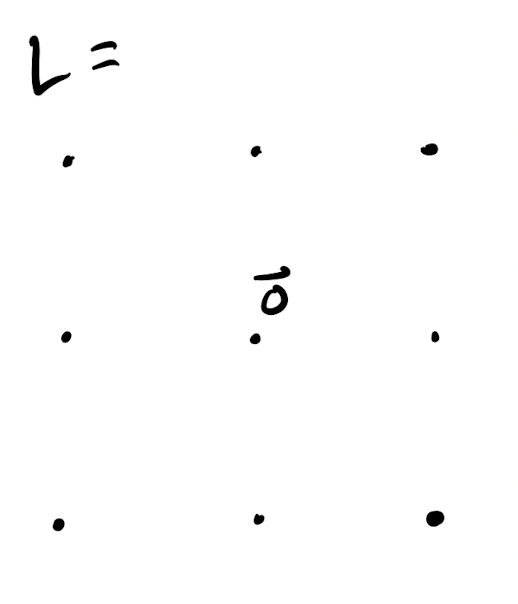
\includegraphics[width=4cm]{Lecture Files and Images/lec15-L0.png}
\end{center}
\end{example}

As we can see in the example, by using the projection $\pi,$ each $G$ can be decomposed into a discrete point group $\overline{G}$ isomorphic to $C_n$ or $D_n$, and a discrete group $L \subseteq \RR^2$, classified in Theorem \ref{discrete sub of r2}. In fact, we can constrain the possibilities even more! The following proposition is a start.

\begin{proposition}
Every $A \in \overline{G}$ maps $L$ to $L.$
\end{proposition}
\begin{proof}
Next time!
\end{proof}

%add another example?

\newpage